\documentclass[10pt,article]{article}
\usepackage{pdfpages}
\usepackage[letterpaper,margin=0.3in]{geometry}
\usepackage{graphicx}
\usepackage{booktabs}
\usepackage{url}
\usepackage{enumitem}
\usepackage{palatino}
\usepackage{tabularx}
\fontfamily{SansSerif}
\selectfont

\usepackage[UTF8]{ctex}
\usepackage[T1]{fontenc}
\usepackage
%[ansinew]
[utf8]
{inputenc}

\usepackage{color}
\definecolor{mygrey}{gray}{0.82}
\textheight=9.75in
\raggedbottom

\setlength{\tabcolsep}{0in}
\newcommand{\isep}{-2 pt}
\newcommand{\lsep}{-0.5cm}
\newcommand{\psep}{-0.6cm}
\renewcommand{\labelitemii}{$\circ$}

\pagestyle{empty}
%-----------------------------------------------------------
%Custom commands
\newcommand{\resitem}[1]{\item #1 \vspace{-2pt}}
\newcommand{\resheading}[1]{{\small \colorbox{mygrey} { \begin{minipage}{0.99\textwidth}\centering{\textbf{#1 \vphantom{p\^{E}}}}\end{minipage}}}}
\newcommand{\ressubheading}[3]{
	\begin{tabular*}{6.62in}{l @{\extracolsep{\fill}} r}
		\textsc{{\textbf{#1}}} & \rightline\textsc{\textit{[#2]}} \\
	\end{tabular*}\vspace{-8pt}}
%-----------------------------------------------------------

\begin{document}
	
	\begin{table}[h]
		\begin{minipage}{0\linewidth}
			\centering
			
\includegraphics[height =0.8in]{./whulogo.png}
		\end{minipage}
		\begin{minipage}{0.9\linewidth}
			%\centering
			\setlength{\tabcolsep}{70pt}
			\def\arraystretch{1.1}
			\begin{tabular}{ll}
				\textbf{\Large{易守拙}}  &  {手机:+86 13667280239} \\
				\textbf{计算机学院,计算机弘毅班} &  {邮箱:yishouzhuo@whu.edu.cn} \\
				\textbf{武汉大学}
			\end{tabular}
		\end{minipage}
		\begin{minipage}{0\linewidth}
			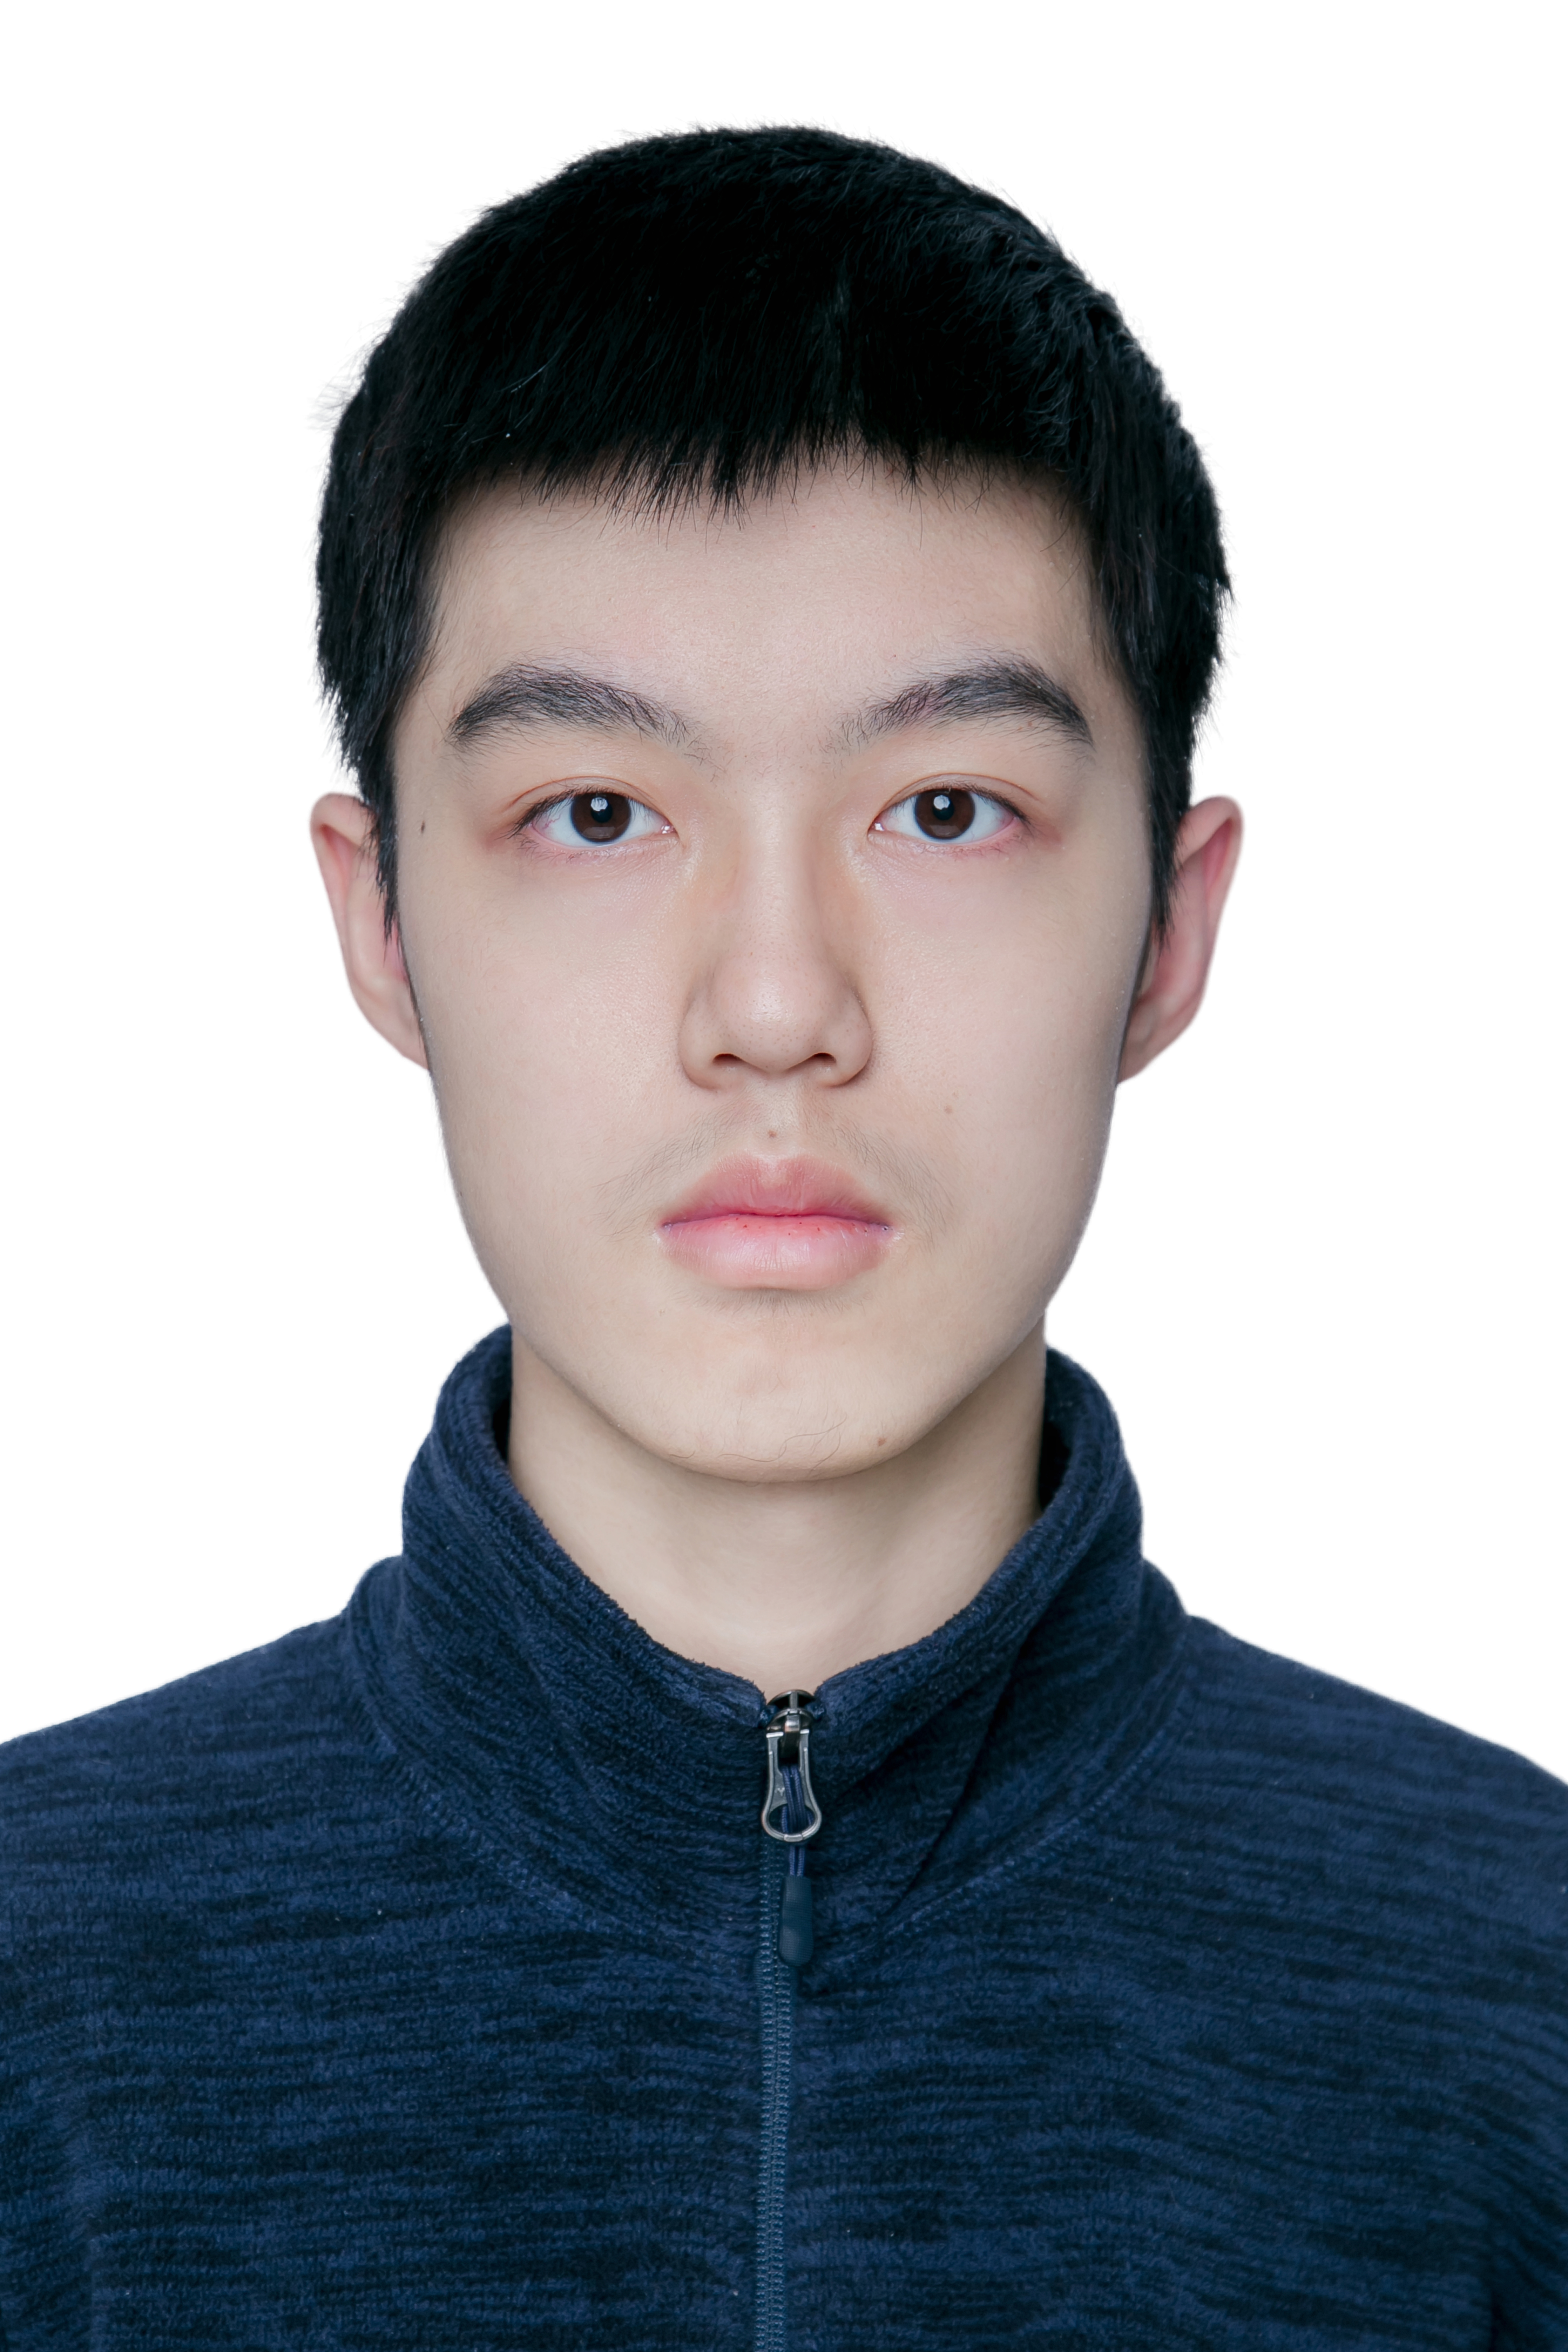
\includegraphics[height =1in]{photo.png}
		\end{minipage}\hfill
	\end{table}
	
	\noindent
	\resheading{\textbf{校内成绩}}\\[-0.5cm]
	\begin{itemize}
		\setlength\itemsep{-0.45em}
		\item 主修专业:计算机科学与技术(计算机弘毅班) \hfill {[2024 - 2028]}
		\\绩点:3.87/4.00(5/29)  
		\\均分:92.65/100(5/29)
		\\CET-4: 608 \quad CET-6: 557
		\\修读的专业课和成绩:高级语言程序设计A(97),数据结构A(97),计算机组成与体系结构A(85),操作系统A(91),算法设计与分析(96)
		\\[-0.6cm]
	\end{itemize}
	
	
	\noindent
	\resheading{\textbf{科研经历}}\\[-0.45cm]
	\begin{itemize}
		\setlength\itemsep{-0.2em}
		
		\item \textbf{武汉大学智能感知与机器学习研究组(SIGMA)}\hfill {[2025.1-2025.7]}
		\begin{itemize}[noitemsep,nolistsep]
			\item 指导老师：童旅杨博士后(武汉大学计算机学院)
			\item 项目类别：大学生创新创业项目
			\item 研究内容：基于胎儿先心病的多模态可解释性模型
			\item 研究成果：省级大创项目成功结题
		\end{itemize}
		
		\item \textbf{武汉大学智能感知与机器学习研究组(SIGMA)}\hfill {[2025.9-2026.7]} 
		\begin{itemize}[noitemsep,nolistsep]
			\item 指导老师：刘友发副研究员(武汉大学计算机学院)
			\item 研究内容：基于大型视觉语言模型的无源迁移学习
			\item 研究成果：一篇学术论文在撰
		\end{itemize}
        \item \textbf{中国科学院大学机器学习与感知实验室(LAMP)}\hfill {[2026.7-至今]} 
		\begin{itemize}[noitemsep,nolistsep]
			\item 指导老师：张同长聘助理教授(中国科学院大学电子电气与通信工程学院)
			\item 研究内容：世界模型
		\end{itemize}
		
	\end{itemize}
	\noindent
	\resheading{\textbf{项目经历}}\\[-0.45cm]
	\begin{itemize}
		\setlength\itemsep{-0.2em}
	
		
		\item \textbf{字节跳动工程训练营——故事成片 Story-to-video}\hfill {[2025.12]} 
		\begin{itemize}[noitemsep,nolistsep]
			\item 实现了“自然文本输入到视频产出”的全链路自动化,实现可视化分镜管理、单镜头编辑,并整合了图像生成、动态视频渲染及AI配音技术
			\item 在小组中参与了后端LLM/TTS等模型部署工作以及后端与服务端通信链路的设计
			\item 字节跳动工程训练营成功结营
		\end{itemize}
		
	\end{itemize}
	
	\noindent
	\resheading{\textbf{我的技能 
			%	\& 我的科研兴趣
	}}\\[-0.5cm]
	\begin{itemize}
		\item 掌握Python/Pytorch工具,在前期科研训练中积攒了一定的从idea出发到代码、实验、调参的能力\\[-0.7cm]
		\item 掌握ssh/\LaTeX 等所需的基本技能 \\[-0.7cm]
	\end{itemize}
	
	
	\noindent
	\resheading{\textbf{获得的奖项}}\\[-0.2cm]
	\begin{itemize}[noitemsep,nolistsep]
		
		\item \textbf{2026雷军计算机本科生奖学金}\hfill {[校级]}\\[-0.4cm]
		

		
		\item \textbf{2024-2025第十六届蓝桥杯省赛 C/C++ 大学 A 组二等奖}\hfill {[省级]}\\[-0.4cm]
		
		% \item \textbf{2024-2025第十七届华中杯大学生数学建模挑战赛二等奖}\hfill {[省级]}\\[-0.4cm]
		
		
		
		\item \textbf{2025-2026全国大学生数学竞赛非数学A类二等奖}\hfill {[省级]}\\[-0.4cm]
		
		\item \textbf{2025-2026第二届CCF算法能力大赛二等奖（并入围决赛）}\hfill {[省级]}\\[-0.4cm]
		\item \textbf{2025-2026 中国高校计算机大赛-团体程序设计天梯赛全国三等奖}\hfill {[国家级]}\\[-0.4cm]
		\item \textbf{2026 全国大学生计算机系统能力大赛-操作系统设计赛(全国)-OS内核实现赛道 全国二等奖}\hfill {[国家级]}\\[-0.4cm]
		
	\end{itemize}
	
	
	\noindent
	\resheading{\textbf{自我评价}}\\[-0.2cm]
	\begin{itemize}[noitemsep,nolistsep]
		\item{\textbf{具有良好的数学理解力与较强的理论学习能力,学习主动,适应能力强,期望在有挑战性的研究工作中将理解转化为实际贡献,证明自己的科研能力}}\\[-0.4cm]
	\end{itemize}
	
	%\includepdf[pages=1]{GPA大二下.pdf}
\end{document}